\section{Methoden}

\subsection{Allgemeine Funktionsweise eines Spektrographen}
Mit Hilfe eines Spektrographen kann man Licht in seine Farben zerlegen. Dabei besteht ein Spektrograph im Wesentlichen aus folgenden Komponenten:

\begin{itemize}

\item Teleskop: Das Teleskop wird benötigt, um Licht zu sammeln und es zu fokussieren.

\item Spalt: Der Spalt schirmt unerwünschte Störquellen ab und sorgt dafür, dass am Dispersionselement ankommende Strahlung im besten Fall von einem Punkt ausgeht, da sich sonst die Auflösung verringert. Dabei kann die Spaltbreite allerdings nicht beliebig klein gewählt  werden, da dadurch natürlich auch die Intensität des Lichts abnimmt. Deshalb muss hier ein Optimum gefunden werden.

\item Kollimator: Der Kollimator ist eine Linse, die aus dem einfallenden Licht paralleles Licht erzeugt.

\item Dispersionselement: Das Dispersionselement ist der Hauptbestandteil des Spektrographen. Es trennt das Licht in Abhängigkeit von der Frequenz. Dabei kann es ein Prisma, oder auch ein Gitter sein. (Das Prisma trennt das Licht auf Grund der Frequenzabhängigkeit der Brechung, während die Trennung beim Gitter durch Interferenzeffekte hervorgerufen wird.)

\item Kamera-Objektiv: Das Kamera-Objektiv wird benötigt, um das durch das Dispersionselement erzeugte Spektrum auf den CCD-Detektor abzubilden.

\item CCD-Detektor: Der CCD-Detektor nimmt das Bild auf und digitalisiert es.

\end{itemize}
Im Bamberger Spektrographen wird ein Blaze-Reflektionsgitter verwendet. (siehe Abb. \ref{fig:101} und \ref{fig:102} ) Dieses hat regelmäßig angeordnete geneigte Furchen und bietet so den Vorteil, dass das Intensitätsmaximum in Richtung des dispergierten Lichtes verschoben wird. Laut \cite{ronomischesPraktikum} ergibt sich aus der Bedingung für konstruktive Interferenz und dem Huygensschen Prinzip:

\begin{equation}
d \cdot ( \sin(\alpha) + \sin(\beta) ) = \Delta s \overset{!}{=} n \cdot \lambda
\label{form:Interferenz}
\end{equation}
Dabei sind $\alpha$, $\beta$ und d wie in den Abb. \ref{fig:101} und \ref{fig:102} zu erkennen. $\Delta s$ ist  die Wegdifferenz, n die Beugungsordnung und $\lambda$ die Wellenlänge des Lichts. Mit Hilfe dieser Formel kann man durch Messung von $\beta$ $\lambda$ bestimmen.

Um die Qualität  eines Spektrums zu beurteilen, wird das spektrale Auflösungsvermögen $R$ mittels der Wellenlänge $\lambda$ und der zugehörigen Unschärfe $\Delta \lambda$ folgendermaßen definiert:

\begin{equation}
R = \frac{\lambda}{\Delta \lambda}
\end{equation}

\newpage

Die Unschärfe $\Delta \lambda$  wird  dabei durch zwei Prozesse erzeugt:

\begin{itemize}

\item Beim Beugen des Lichts am Gitter kommt es zum Verwaschen der Linien. Das Auflösungsvermögen des Gitters beträgt $ R_{Gitter} = n \cdot N $, wobei $ N $ die Anzahl der beleuchteten Spalten ist.

\item Die Breite des Spalts führt dazu, dass beliebig nahe Punkte im Spektrum nicht mehr getrennt werden können. 

\end{itemize}

\begin{figure}
		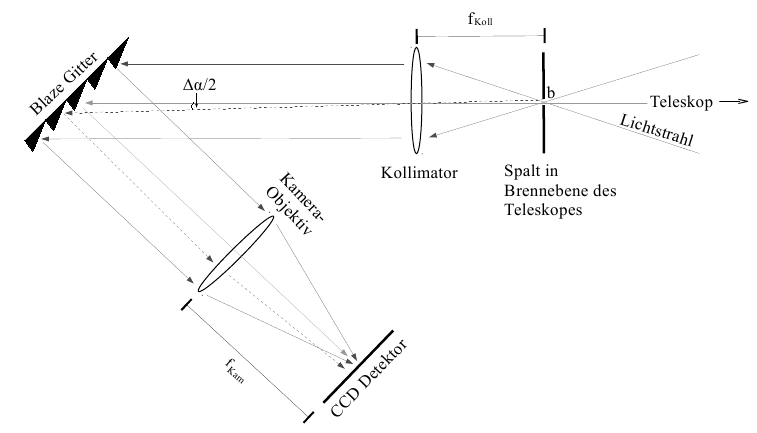
\includegraphics[width=.9\textwidth]{images/Abbildung101}
\caption{ Schematischer Aufbau eines Gitterspektrographen mit Blaze-Gitter (Abbildung entnommen aus \cite{ronomischesPraktikum})}
\label{fig:101}
\end{figure}
\begin{figure}

        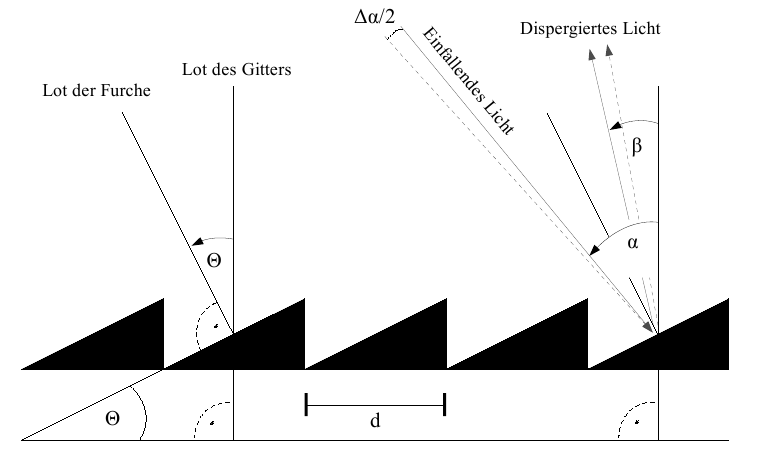
\includegraphics[width=.9\textwidth]{images/Abbildung102.png}
\caption{ Beispiel eines Blaze-Gitters und seiner charakteristischen Größen (Abbildung entnommen aus \cite{ronomischesPraktikum}) }
\label{fig:102}
\end{figure}
\begin{figure}

        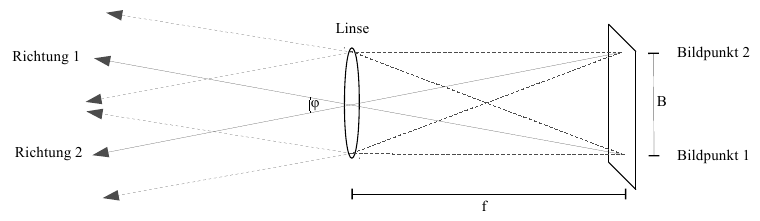
\includegraphics[width=.9\textwidth]{images/Abbildung103.png}
\caption{ Abbildungsmaßstab einer Linse (Abbildung entnommen aus \cite{ronomischesPraktikum})}
\label{fig:103}
\end{figure}

\subsection{Die Rolle des Spalts}
Da der Spalt nicht unendlich schmal ist, trifft das Licht nicht perfekt parallel auf das Gitter. Deshalb variiert der Einfallswinkel $ \alpha $ um $ \Delta \alpha $, was letztendlich das Auflösungsvermögen verschlechtert.

\subsubsection{Wellenlängenunschärfe hervorgerufen durch endliche Spaltbreiten}
Für eine Linse (siehe Abb. \ref{fig:103}) gilt mit Hilfe der Kleinwinkelnäherung:

\begin{equation}
B = 2\cdot \sin{\frac{\phi}{2}} \cdot f = 2 \cdot \frac{\phi}{2} \cdot f = f \cdot \phi
\label{form:Kleinwinkel}
\end{equation}
Der vom Spalt \enquote{umspannte} Winkelbereich $\Delta \alpha $ beträgt nach \eqref{form:Kleinwinkel}:
\begin{equation}
\Delta \alpha = \frac{b}{f_{koll}}
\end{equation}
Leitet man \eqref{form:Interferenz} nach $ \alpha $ ab, erhält man:

\begin{equation}
\frac{d \lambda}{d \alpha} = \frac{d}{n} \cdot \cos{\alpha}
\end{equation}
Für hinreichend kleine $\alpha$ ergibt sich mit der Näherung $ \Delta \lambda = \frac{d\lambda}{d\alpha} \cdot \Delta \alpha $ :

\begin{equation}
\Delta \lambda = \frac{d}{n} \cdot \cos{\alpha} \cdot \frac{b}{f_{koll}}
\end{equation} 
Für das Auflösungsvermögen des Spalts ergibt sich mit $ R = \frac{\lambda}{\Delta \lambda} $ die Formel:

\begin{equation}
R_{Spalt} = \frac{n \cdot f_{Koll}}{d \cdot b \cdot \cos \alpha} \lambda
\end{equation}
Also ist die Auflösung auch durch den Spalt auf einen endlichen Wert begrenzt.

\subsubsection{Auflösung des Spektrographen}
Laut \cite{ronomischesPraktikum} ist die durch die Spaltbreite vorgegebene Auflösung typischerweise wesentlich kleiner als die des Gitters. Deshalb kann in guter Näherung davon ausgegangen werden, dass für die Auflösung des gesamten Spektrographen gilt:

\begin{equation}
R = \frac{n \cdot f_{Koll}}{d \cdot b \cdot \cos \alpha} \lambda
\label{form:Auflösung}
\end{equation}
Um eine möglichst gute Auflösung zu erhalten, muss man also die Parameter aus \eqref{form:Auflösung} so wählen, dass $ R $ möglichst groß wird. Dies ist in der Praxis jedoch nur bedingt möglich. Die zwei einfachsten Maßnahmen, dies umzusetzen sind:

\begin{itemize}

\item Verkleinern der Spaltbreite $ b $

\item Beobachten in hohen Beugungsordnungen $ n $

\end{itemize}

\subsubsection{Optimierung der Auflösung des Spektrographen}
Beide oben genannten Maßnahmen bringen auch Nachteile mit sich. So darf z.B. die Spaltbreite nicht zu klein gewählt werden, da Sterne die von der Erde aus beobachtet werden durch das Seeing eine nicht zu vernachlässigende Ausdehnung erhalten. Ein Stern beim durchschnittlichen Bamberger Seeing hat in der Fokalebene einen Durchmesser von $48.9 \mu \mathrm{m} $. Dieser Wert wäre also der kleinste mögliche Wert mit voller Lichteinstrahlung und somit der ideale Wert für die Blendenöffnung.

\newpage

\subsection{Echelle-Spektrograph}
\subsubsection{Überlappung von Beugungsordnungen}
Verwendet man hohe Beugungsordnungen, überlappen sich diese meistens sehr stark. Im Folgenden soll als Beispiel berechnet werden, für welche Wellenlängen der Ordnungen $ n = $ 34, 46 und 58 Licht unter dem gleichen Ausfallswinkel  $ \beta $ gebeugt wird wie Licht der Wellenlänge $ \lambda_{33} = $ 6662.2686 $ \AA $ in der Ordnung $ n = $ 33. (Dabei sollen der Einfallswinkel $ \alpha $ und der Spaltabstand konstant gehalten werden.)\\

Da $\alpha$ und $d$ konstant gehalten werden und $\beta$ konstant sein soll, muss für das Licht verschiedener Wellenlängen $n_1 \cdot \lambda_1 = n_2 \cdot \lambda_2$ gelten. Somit folgt: 

\begin{equation}
\lambda_n = \frac{33}{n} \cdot \lambda_{33}.
\end{equation}
Dies ergibt für n = 34 $\lambda_{34} \approx 6466.3195 \AA$, für n = 46 $\lambda_{46} \approx 4779.4536 \AA$ und für n = 58 $\lambda_{56} = 3790.6011 \AA$.\\

Um diese Überlagerungen aufzuspalten, wird ein Echelle-Spektrograph verwendet.

\subsubsection{Funktionsweise eines Echelle-Spektrographen}

\begin{figure}
		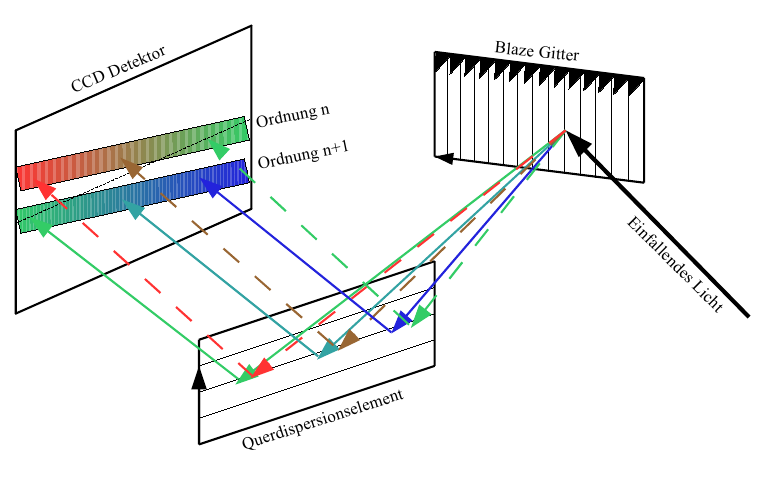
\includegraphics[width=.9\textwidth]{images/Abbildung104}
\caption{ Prinzip eines Echelle-Spektrographen (Abbildung entnommen aus \cite{ronomischesPraktikum})}
\label{fig:104}
\end{figure}

\begin{table}
		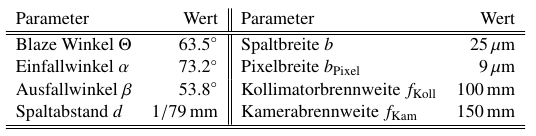
\includegraphics[width=.9\textwidth]{images/Tabelle101}
\caption{ Eigenschaften des im Praktikum verwendeten Echelle-Spektrographen (Tabelle entnommen aus \cite{ronomischesPraktikum})}
\label{tab:Echelle}
\end{table}

Das zusätzliche Element eines Echelle-Spektrographen ist ein weiteres Beugungsgitter, das allerdings senkrecht zur Beugungsrichtung des ersten Gitters angebracht wird. Dadurch spalten sich die z.B. horizontal verschmierten Beugungsordnungen in vertikaler Richtung auf und das Spektrum kann mit Hilfe eines CCD-Chips und anschließender Reduktion der Daten erzeugt werden. Da $ \alpha + \beta = 2 \Theta $ (siehe Abb. \ref{fig:102}), folgt mit der zugehörigen als Blaze-Wellenlänge bezeichneten Wellenlänge $ \lambda_n^0 $:

\begin{equation}
n \lambda_n^0 = d ( \sin(\alpha) + \sin(\beta) ) \vert_{\alpha + \beta = 2 \Theta} = d ( \sin(\alpha) + \sin(2 \Theta - \alpha) )
\end{equation} 

Ersetzt man $\lambda$ aus \eqref{form:Auflösung} durch $ \lambda_n^0 $, erhält man laut \cite{ronomischesPraktikum} eine sehr gute Näherung für die Auflösung $ R_{Echelle} $. Das Ersetzen liefert:

\begin{equation}
R_{Echelle} = \frac{n\cdot f_{Koll}}{d\cdot b\cdot cos \alpha}\cdot \frac{d}{n}[sin \alpha + sin(2\Theta-\alpha)] = \frac{f_{Koll}}{b}\cdot \left[tan \alpha + \frac{sin(2\Theta-\alpha)}{cos \alpha}\right]
\label{form:R_Echelle}
\end{equation}
Dieser Term enthält nur Variablen, die sich aus dem Versuchsaufbau als konstant ergeben. Damit ergibt sich $ R_{Echelle} $ mittels Einsetzen der Werte aus Tabelle \ref{tab:Echelle} zu:

\begin{equation}
R_{Echelle} = \frac{100 \cdot 10^{-3}m}{25 \cdot 10^{-6}m}\cdot \left[tan (73.2^{\circ}) + \frac{sin(53.8^{\circ})}{cos (73.2^{\circ})}\right] \approx 24416
\end{equation}

\subsection{Auflösung des CCD-Chips}
Die gesamte Auflösung des Aufbaus ist natürlich nur ungefähr so gut, wie das Bauteil mit der schlechtesten Auflösung. Deshalb ist es nur dann sinnvoll die Auflösung eines Bauteils zu verbessern, wenn alle anderen eine ähnliche oder bessere Auflösung besitzen. Ist dies nicht der Fall, sollten zuerst die schlechteren Bauteile verbessert werden. Daher ist es auch sinnvoll sich über die Auflösung des CCD-Chips Gedanken zu machen.\\

Das Nyquist-Kriterium besagt nach \cite{ronomischesPraktikum}, dass das räumliche Auflösungselement des CCDs durch die zweifache Pixelbreite $ b_{Pixel} $ gegeben ist. Ersetzt mal also aufgrund des Nyquist-Kriteriums die Größe b durch $ 2b_{Pixel} $, ergibt sich:

\begin{equation}
R_{CCD} = \frac{f_{Kamera}}{2b_{Pixel}}\cdot \left[tan \beta + \frac{sin(2\Theta-\beta)}{cos \beta}\right]
\end{equation}

Einsetzen von Tabellenwerten aus Tabelle \ref{tab:Echelle} liefert:
 
\begin{equation}
R_{CCD} = \frac{150\cdot10^{-3}m}{18\cdot10^{-6}m}\cdot \left[tan (53.8^{\circ}) + \frac{sin(73.2^{\circ})}{cos (53.8^{\circ})}\right] \approx 25000
\end{equation}

Also ist die Auflösung der CCD-Kamera optimalerweise in der gleichen Größenordnung wie die des Spektrographen.
			
\subsection{Durchführung der Messung}
Die Hauptaufgabe dieses Experiments war es ein Sonnen- und ein Sternspektrum aufzunehmen und auszuwerten. Im folgenden wird ausgeführt, wie dabei vorgegangen wurde.

\subsubsection{Messung eines Sonnenspektrums}
Bei der Messung des Sonnenspektrums wurde zuerst ein Spektrum mit der Thorium-Argon-Lampe, dann das Sonnenspektrum und schließlich wieder das der Thorium-Argon-Lampe aufgenommen, um sichergehen zu können, dass die Messung korrekt funktioniert hat. Mit der Thorium-Argon-Lampe wurde 45 Sekunden lang belichtet, während bei der Messung des Sonnenspektrums natürlich wesentlich kürzer belichtet werden musste.

Dabei durfte das Teleskop unter keinen Umständen direkt auf die Sonne zeigen, da der Spektrograph sonst durch die starke Sonnenstrahlung beschädigt werden hätte können!

\subsubsection{Messung eines Sternspektrums}
Bei der Messung des Sternspektrums musste zuerst das zu messende Objekt mit dem Sucher gefunden und mit der Kamera eingestellt werden. Dies stellte sich als problematisch heraus, da der Sucher nicht genau auf das Teleskop eingestellt war. Als das Objekt richtig eingestellt war, wurde zunächst eine 45-sekündige Aufnahme mit der Thorium-Argon-Lampe durchgeführt. Dann wurden jeweils 5-minütige Aufnahmen eines Darkframes und des Sternspektrums und schließlich wieder eine 45-sekündige Aufnahme mit der Thorium-Argon-Lampe durchgeführt.

\subsection{Datenreduktion}
Um die aufgenommenen Spektren am Computer untersuchen zu können, müssen sie zunächst kalibriert und reduziert werden. Dies wurde in diesem Versuch mit dem Programmpaket MIDAS (Munich Image Data Analysis System) durchgeführt. Zunächst wurden die Beugungsordnungen und deren Position auf dem CCD-Chip identifiziert. Dazu mussten mehrere Kalibrationen mit verschiedenen angegebenen Anzahlen von Beugungsordnungen durchgeführt werden, bis alle Beugungsordnungen korrekt identifiziert wurden. Der zweite Schritt bestand darin, den Pixeln auf dem CCD-Chip die entsprechenden Wellenlängen zuzuordnen. Dazu wurde das aufgenommene Spektrum der ThAr-Lampe mit einem Referenzspektrum verglichen, indem zwei im Referenzspektrum gegebene Linien und deren Beugungsordnungen in dem aufgenommenen Spektrum markiert wurden. Anhand dieser Daten konnte MIDAS dann die Wellenlängenkalibration durchführen.\
Die eigentliche Reduktion der Daten wurde danach vorgenommen. In der Reduktion werden CCD-Effekte (Dunkelstrom, überbelichtete Pixel aufgrund von hochenergetischer kosmischer Strahlung) und in dem optischen Aufbau entstehendes Streulicht von der Aufnahme entfernt. Weiterhin wird eine Wellenlängenkalibration anhand des ThAr-Vergleichsspektrums durchgeführt und die einzelnen Beugungsordnungen extrahiert und in eindimensionale Datenarrays umgewandelt (\enquote{rebinning}). Es ist außerdem notwendig, den Einfluss der Blaze-Funktion durch eine Flatfield-Korrektur zu entfernen, um ein lückenloses Spektrum zu erzeugen. Schließlich werden noch die einzelnen Beugungsordnungen zu einem einzelnen Spektrum zusammengefügt und das kontinuierliche Spektrum auf eins normiert. Die Normierung wurde für unsere Messung jedoch nicht durchgeführt.  